\documentclass[xcolor={dvipsnames},10pt]{beamer}

\usepackage{../style.sty/mybeamer}

\title[Industriedynamik]{Übung Industriedynamik}
\author{Dominic Görz, Daniel Horstmann}
\date{\today}
\setbeamertemplate{navigation symbols}{}%remove navigation symbols

\begin{document}

\begin{frame}
  \maketitle
\end{frame}

\begin{frame}{Contents}
  \tableofcontents
\end{frame}

\section{Aufgabe 1}

\subsection{Gewinne}

\subsubsection{Gewinne 1 a)}
\begin{frame}{Profite 1a)}
\begin{columns}[T]
    \begin{column}{.3\textwidth}
      \begin{itemize}
      \item Der Gewinn einer Firma steigt
      \item Die Gewinne der anderen Firmen fallen und erreichen den Wert Null
      \end{itemize}
      \end{column}
      \begin{column}{.7\textwidth}
      \begin{figure}[t]
            \centering
            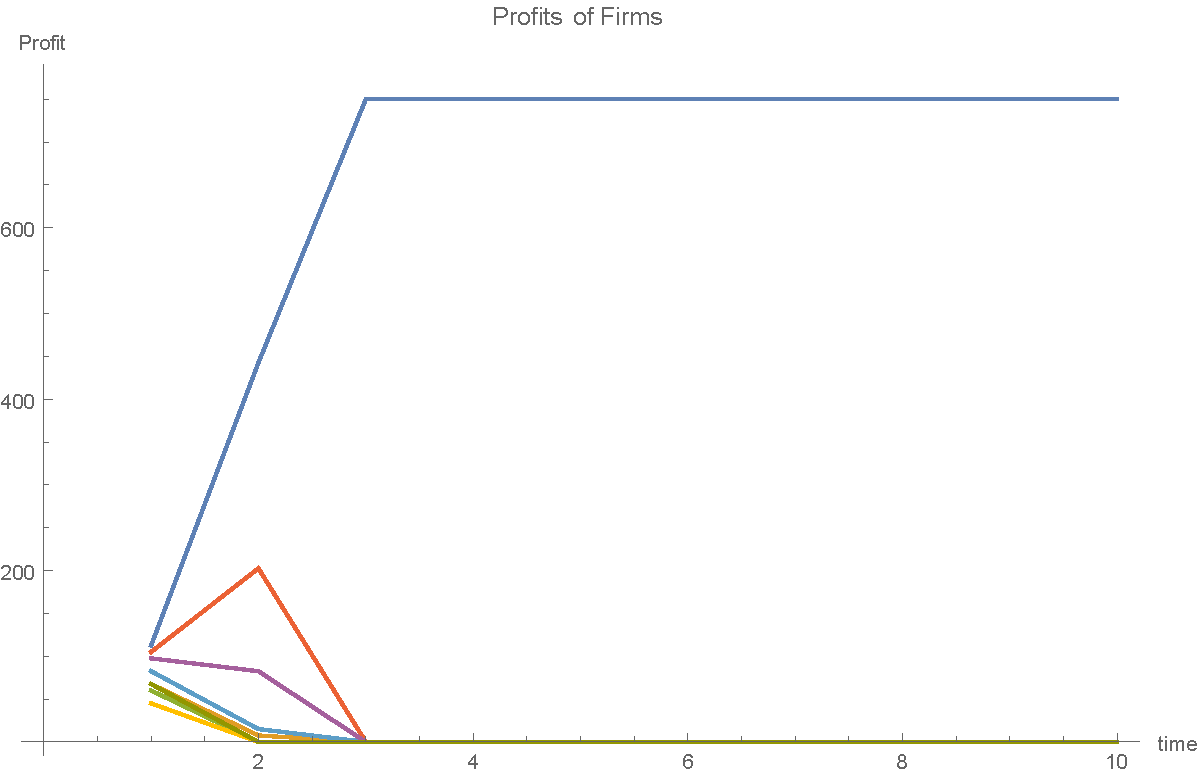
\includegraphics[scale=0.35]{../Plots/profit1a}
            \caption{Profite in 1 a)}
            \label{fig:profit1a}
       \end{figure}
    \end{column}
  \end{columns}
\end{frame}

\subsubsection{Gewinne 1 b)}
\begin{frame}{Profite 1b)}
\begin{columns}[T]
    \begin{column}{.3\textwidth}
      \begin{itemize}
      \item Die Gewinne der Firmen, welche die smarte Komponente einkaufen,
            scheinen um einen Mittelwert zu fluktuieren.
      \item Die Gewinne der Firmen, welche die smarte Komponente selber herstellen,
            sinken und erreichen den Wert Null
      \end{itemize}
      \end{column}
      \begin{column}{.7\textwidth}
      \begin{figure}[t]
            \centering
            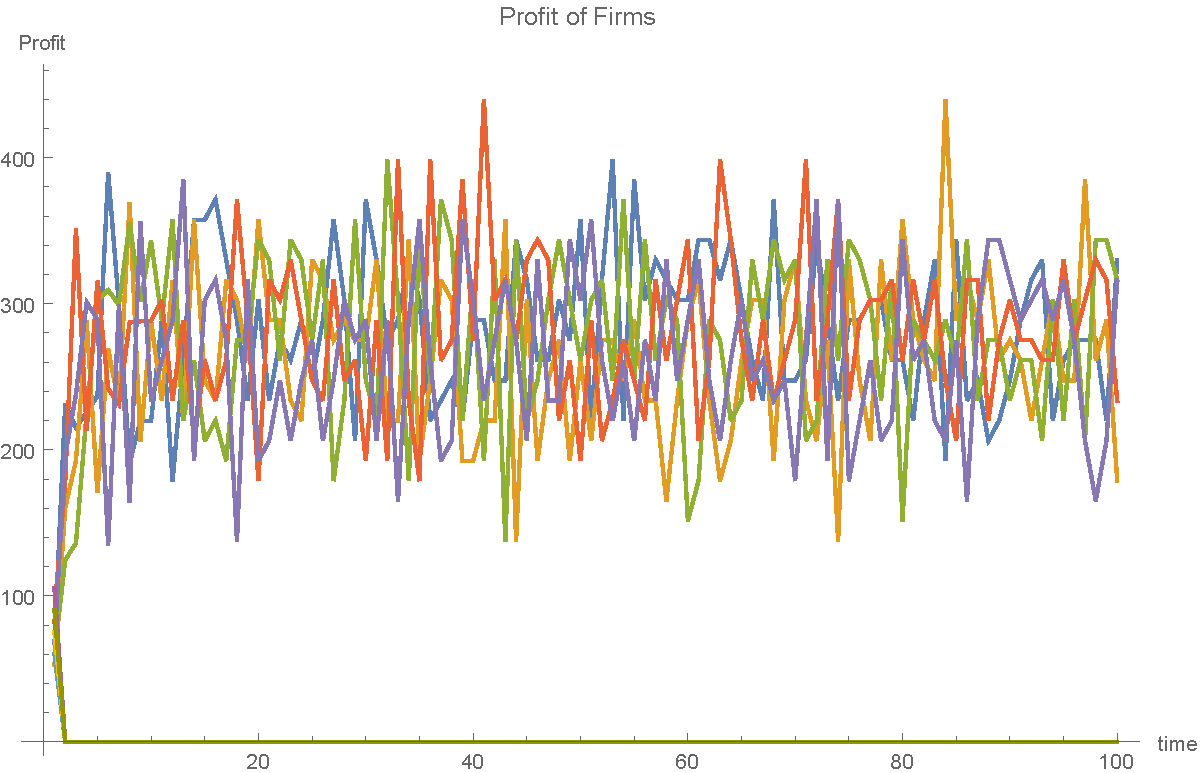
\includegraphics[scale=0.35]{../Plots/profit1b}
            \caption{Profite in 1 b)}
            \label{fig:profit1b}
       \end{figure}
    \end{column}
  \end{columns}
\end{frame}

\subsubsection{Gewinne 1 c)}
\begin{frame}{Profite 1c)}
\begin{columns}[T]
    \begin{column}{.3\textwidth}
      \begin{itemize}
      \item Die Gewinne aller Firmen scheinen um einen Mittelwert zu fluktuieren.
      \end{itemize}
      \end{column}
      \begin{column}{.7\textwidth}
      \begin{figure}[t]
            \centering
            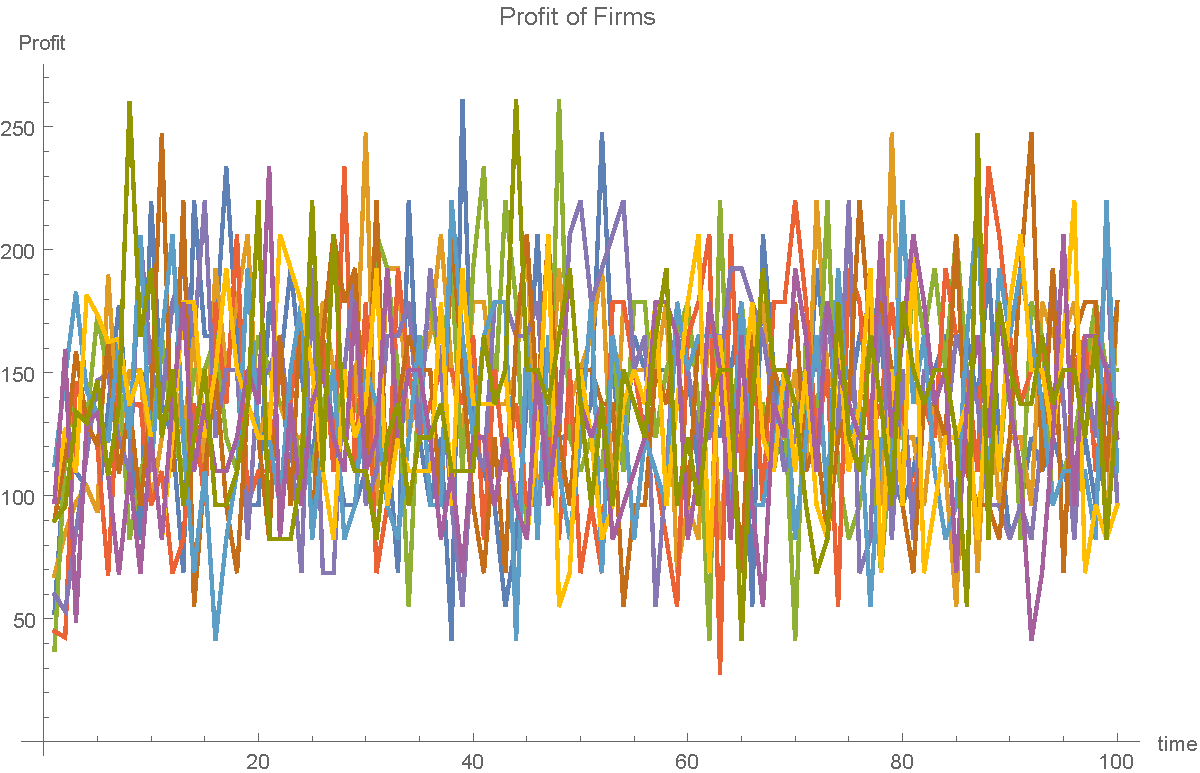
\includegraphics[scale=0.35]{../Plots/profit1c}
            \caption{Profite in 1 c)}
            \label{fig:profit1c}
       \end{figure}
    \end{column}
  \end{columns}
\end{frame}

\section*{}
\begin{frame}
\centering
 Vielen Dank für die Aufmerksamkeit!
\end{frame}

\end{document}